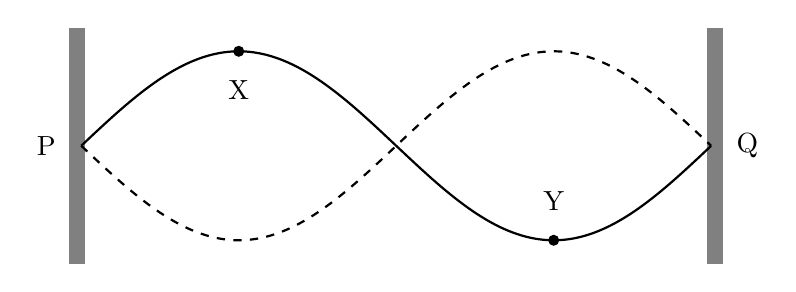
\begin{tikzpicture}
  % walls
  \fill[gray] (-0.15,-1.5) rectangle (0.05,1.5);
  \fill[gray] (7.95,-1.5) rectangle (8.15,1.5);
  \node[left] at (-0.2,0) {P};
  \node[right] at (8.2,0) {Q};
  % solid standing-wave shape (one wavelength)
  \draw[thick,smooth,samples=100,domain=0:8] plot (\x,{1.2*sin(45*\x)});
  % dashed opposite phase
  \draw[thick,dashed,smooth,samples=100,domain=0:8] plot (\x,{-1.2*sin(45*\x)});
  % marked points
  \fill (2,1.2) circle (2pt);
  \fill (6,-1.2) circle (2pt);
  \node[below] at (2,0.95) {X};
  \node[above] at (6,-0.95) {Y};
\end{tikzpicture}
